% Para adicionar uma imagem ou incluir um arquivo .tex você precisa 
% adicionar \CWD
% caminho relativo (ao documento principal) do diretório.
% 
% Exemplo:
% \begin{figure}
%   \includegraphics{\CWD/imagens/exemplo.pdf}
% \end{figure}


In the problem we are tasked to find a \textbf{convex combination} of the input's points which gives as a result a given query point, for several queries. As the name suggest, it is related to \textit{convex sets theory}, furthermore, it is possible possible to do so \textbf{if and only if} the point is contained inside the convex hull of the given set of points (proof to this fact is the base of convex sets theory and can be found in any related bibliography).

We already know when it's possible or not to find such combinations, just remains to find the actual combination in a positive case. Note that we just need to find a triangle from the convex hull containing the point, since a triangle is a convex polygon and if the point is inside the convex hull then it is inside at least one of its triangles.

Let's suppose we found such triangle:

\begin{figure}[!tbh]
	\centering
	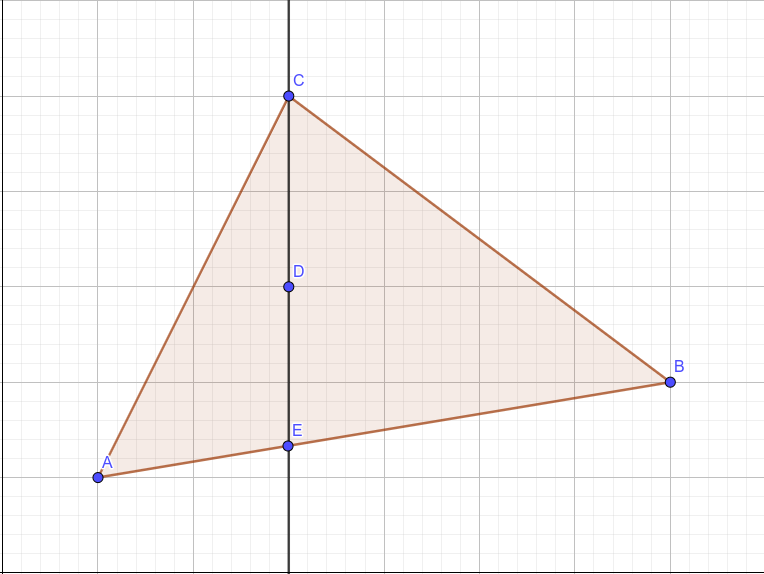
\includegraphics[width=0.5\linewidth]{\CWD/images/a.png}
\end{figure}

where $D$ is the query point. We can extend line $\overline{CD}$ and mark point $E$. 

From the vector equation of the line it follows that $\exists t \in [0, 1]: D = (1 - t) \cdot C + t \cdot E$. The same way $\exists k \in [0, 1]: E = k \cdot A + (1 - k) \cdot B$. Combining both results we get
	$$D = (1 - t) \cdot C + t \cdot k \cdot A + t \cdot (1 - k) \cdot B$$

which is a convex combination of points $A, B$ and $C$ \big(you may check $(1 - t) + t \cdot k + t \cdot (1 - k) = 1$\big).

In order to fit time constrains we need to find the triangle in a clever way, an idea is with binary search over the diagonals with one of the points fixed. With this approach we get a time complexity of $\mathcal{O}((n + q) \cdot \log n)$, which is enough to get AC. We never get to use more than $3$ elements in our convex combination.
